%!TEX program = xelatex
\documentclass[cn,hazy,blue,14pt,screen]{elegantnote}
\title{Raiser:平衡机器计算函数优化缓存工具}

\author{施华}
\institute{Computational function optimization cache tool}

\version{beta-0.1}
\date{\zhtoday}

\usepackage{array}

\begin{document}

\maketitle

\centerline{
  
\includegraphics[width=0.2\textwidth]{logo-ae.png}
}



\section{Raiser介绍}

Raiser是一个基于HDF5的优化计算函数的缓存装饰器

Raiser有下面几个特性:

\begin{itemize}
  \item 对原始代码侵入少
  \item 高速
  \item 可扩展其他缓存技术
\end{itemize}

以下主要是主体框架和基础套餐的设计说明



\subsection{主体框架}

Raiser作为计算优化缓存工具,主要提供了对numpy的ndarray数据帧的缓存优化支持。相关模块技术列表如下

\begin{enumerate}[label=\arabic*).]
	\item \textit{后端缓存}\\
	基于HDF5设计缓存。
	\item \textit{装饰器}\\
	利用Python特有的装饰器技术
\end{enumerate}

\centerline{
	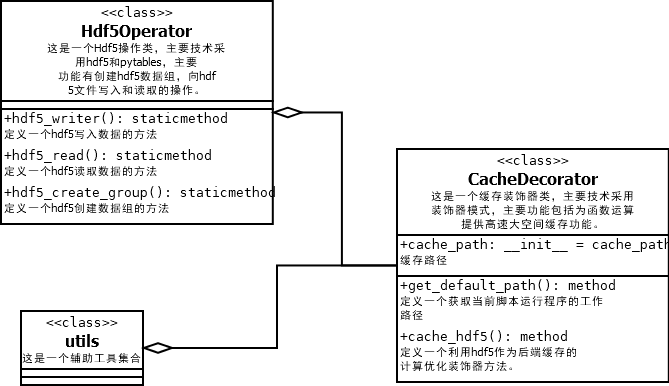
\includegraphics[width=0.8\textwidth]{Raiser.png}
}








\subsection{使用示例}

Raiser的使用。

代码示例:

\begin{lstlisting}
	from Raiser.cache_operator import *
	from Raiser.cache_decorator import *
	import numpy as np 
	
	
	
	### HDF5操作测试 ###########################################
	### hdf5写入数据
	print("########################################################################## 1")
	x = np.array([[1, 2, 3], [4, 5, 6]])
	y = np.array([[1, 2], [3, 4], [5, 6]])
	Hdf5Operator.hdf5_writer_ndarray(h5path = 'test_operator.h5',
	group_name = 'x',
	info = 'var x test',
	version_name = '01',
	ndarray_obj = x)
	Hdf5Operator.hdf5_writer_ndarray(h5path = 'test_operator.h5',
	group_name = 'y',
	info = 'var y test',
	version_name = '01',
	ndarray_obj = y)                                 
	### hdf5读取数据
	print("########################################################################## 2")
	tmp_x = Hdf5Operator.hdf5_read_ndarray(h5path = 'test_operator.h5',
	group_name = 'x',
	version_name = '01')         
	# print(x,type(x))    
	### 缓存装饰器测试 ############################################
	### 获取当前路径
	print("########################################################################## 3")
	CacheDecorator = CacheDecorator(hdf5_name = 'test_operator.h5')
	print(CacheDecorator.cachepath)
	### 定义原始运行函数
	print("########################################################################## 4")
	@CacheDecorator.hdf5_run(storage_name = 'multi_array_result')
	def multi_array(x,y):
	multi_array_result = np.dot(x,y)
	return multi_array_result                                                           
	### 运行函数
	multi_array_result = multi_array(x = 'x',y = 'y')
\end{lstlisting}



\end{document}
